\documentclass[12pt]{article}
\usepackage[utf8]{inputenc}
\usepackage{amsmath}

\title{ECE 3413 Lab 02\\*Polynomials and Transfer Functions}
\author{Leomar Dur\'an}
\date{$9^{\text{th}}$ February 2023}

\usepackage{siunitx}

\usepackage{pdfpages}
\usepackage{minted}
\usepackage{standalone}

\usepackage{mathtools}%
\DeclarePairedDelimiter\brao()%
\DeclarePairedDelimiter\brac[]%
\DeclarePairedDelimiter\braco[)%
\DeclarePairedDelimiter\Brac\{\}%
\DeclarePairedDelimiter\norm\lVert\rVert%
\DeclarePairedDelimiter\piecefn\{.
\DeclarePairedDelimiter\evalat.|

\usepackage{titling}

\usepackage{matlab}
% \newcommand*\matlabtitle\subsection
% \newcommand*\matlabheading\subsubsection
% \newcommand*\mlcell[1]{#1}
% \newenvironment{matlaboutput}{%
    % \minted{matlab}%
% }%
% {%
    % \endminted%
% }%
% \newenvironment{matlabtableoutput}{}{}%

\def\hr{{\par\noindent\rule{\textwidth}{0.4pt}}}

\begin{document}

\maketitle
\newpage

\section{Introduction}

The purpose of this experiment is to serve as a practical introduction to Matlab and Simulink and their graphical user interface.

Matlab is a linear algebra tool, and Simulink is a tool for modeling systems using block diagrams.
They may each be used for modeling control systems among other types of systems.

In this example, we use Matlab to model a polynomial as a row vector of coefficients.
We also use Matlab in conjunction with Simulink to prepare, model and contrast $2$ control systems.

\section{Procedure}

\subsection{Roots and corresponding phase angles of a polynomial}

In this part of the lab, we model a polynomial in Matlab.
This is done by using a row vector.
Of the operations that can be performed on a row vector, $2$ are the \mintinline{matlab}{conv} and \mintinline{matlab}{roots} functions.

\subsubsection{Convolution}\label{sss:conv}

The \mintinline{matlab}{conv} function is used to convolve two vectors representing polynomial multiplication.

For example, we have the polynomials
\[
    \begin{gathered}
        P_1\brao*s = s^2 + 10s + 24\rlap, \\*
        P_2\brao*s = s^4 + 26s^3 + 231s^2 + 766s + 560\rlap. \\*
    \end{gathered}
\]

These may be represented by the row vectors
\[
    \begin{gathered}
        \vec{v}_1 := \brac*{\begin{matrix} 1 & 10 & 24 \\* \end{matrix}}\rlap, \\*
        \vec{v}_2 := \brac*{\begin{matrix} 1 & 26 & 231 & 766 & 560 \\* \end{matrix}}\rlap. \\*
    \end{gathered}
\]

\pagebreak

Then the convolution $\mathbf{v}_1 \ast \mathbf{v}_2$ represents the product $\brao{P_1 P_2}\brao*s$ as follows

\begin{minted}{matlab}
       [   1  26 231 766 560 ]
[ 24  10   1]                         = 1
    [ 24  10   1]                     = 10+26 = 36
        [ 24  10   1]                 = 24 + 260 + 231 = 515
            [ 24  10   1]             = 624 + 2310 + 766 = 3700
                [ 24  10   1]         = 5544 + 7660 + 560 = 13764
                    [ 24  10   1]     = 18384 + 5600 = 23984
                        [ 24  10   1] = 13440
-----------------------------------------------------------------
[1 10 24]*[1 26 231 766 560] = [1 36 515 3700 13764 23984 13440],
\end{minted}

representing the polynomial
\[
    P\brao*s = s^6 + 36s^5 + 515s^4 + 3700s^3 + 13764s^2 + 23984s + 13440\rlap.
\]

\subsubsection{The roots of the polynomial}

The \mintinline{matlab}{roots} function in Matlab returns the roots of the polynomial $P\brao*s$, that is, the values of $s$ s.t. $P\brao*s = 0$.

\subsection{Transfer functions}

In part 2 of the lab, we model a transfer function and modify one of its coefficients to produce a new output.

We use Matlab to set up the parameters for the transfer functions before using Simulink to model them because Matlab allows for a cleaner interface to set up the parameters.

Additionally, we can use Matlab to perform sanity checks along the way because it echos the value of every statement that is not suppressed by the semicolon character (\mintinline{matlab}{;}).

For example, we can echo the poles, zeros, numerators and denominators of the transfer functions to ensure that we set them up correctly.

Simulink is then used to model the system visually as a block diagram.
The transfer functions are compared by their step responses, their response to a step signal.
The signal starts at $\SI1\volt$, then jumpts to $\SI2\volt$ at $\SI1{\milli\second}$.

\subsubsection{Transfer functions in Matlab}

Matlab has transfer function objects.
These can be represented by objects as a ratio of polynomials using the \mintinline{matlab}{tf} function,
or as their zeros, poles and gain using \mintinline{matlab}{zpk}.
In this lab, we make use of the \mintinline{matlab}{tf} objects.

\subsubsection{Poles}

The poles are the roots of the denominator of the transfer function.
Matlab has the function \mintinline{matlab}{pole},
which accepts a transfer function and returns it poles.

\subsubsection{Zeros}

The zeros are the roots of the numerator of the transfer function.
Matlab has the function \mintinline{matlab}{zero},
which accepts a transfer function and returns it zero.

\subsubsection{The modified transfer function}

We are given the transfer function
\[
    H\brao*s = \frac{s^2 + 10s + 24}{s^4 + 26s^3 + 231s^2 + 766s + 560}\rlap.
\]

I have modified it by negating its pole with the minimum magnitude.

\section{Results}

\hr

% This LaTeX was auto-generated from MATLAB code.
% To make changes, update the MATLAB code and export to LaTeX again.

\documentclass{article}

\usepackage[utf8]{inputenc}
\usepackage[T1]{fontenc}
\usepackage{lmodern}
\usepackage{graphicx}
\usepackage{color}
\usepackage{hyperref}
\usepackage{amsmath}
\usepackage{amsfonts}
\usepackage{epstopdf}
\usepackage[table]{xcolor}
\usepackage{matlab}

\sloppy
\epstopdfsetup{outdir=./}
\graphicspath{ {./part01_poles_zeros_mlx_images/} }

\begin{document}

\matlabtitle{Part 1 $-$ Poles and zeros}


\matlabheading{1ab. Roots}

\begin{par}
\begin{flushleft}
Calculate the roots of each of the following polynomials
\end{flushleft}
\end{par}

\begin{matlabsymbolicoutput}
\hskip1em $\displaystyle P_1 =s^6 +s^5 +2\,s^4 +8\,s^3 +7\,s^2 +15\,s+12$
\hskip1em $\displaystyle P_2 =s^6 +s^5 +4\,s^4 +3\,s^3 +7\,s^2 +15\,s+18$
\end{matlabsymbolicoutput}


\begin{par}
\begin{flushleft}
The roots for each polynomial are
\end{flushleft}
\end{par}

\begin{matlabtableoutput}
{
\begin{tabular} {|c|c|c|c|}\hline
\mlcell{ } & \mlcell{CartesianForm} & \mlcell{r} & \mlcell{thetaDeg} \\ \hline
\mlcell{1} & \mlcell{0.9979 + 1.6070i} & \mlcell{1.8916} & \mlcell{58.1624} \\ \hline
\mlcell{2} & \mlcell{0.9979 - 1.6070i} & \mlcell{1.8916} & \mlcell{301.8376} \\ \hline
\mlcell{3} & \mlcell{-1.8615 + 0.0000i} & \mlcell{1.8615} & \mlcell{180} \\ \hline
\mlcell{4} & \mlcell{-0.1302 + 1.4299i} & \mlcell{1.4358} & \mlcell{95.2009} \\ \hline
\mlcell{5} & \mlcell{-0.1302 - 1.4299i} & \mlcell{1.4358} & \mlcell{264.7991} \\ \hline
\mlcell{6} & \mlcell{-0.8739 + 0.0000i} & \mlcell{0.8739} & \mlcell{180} \\ 
\hline
\end{tabular}
}
\end{matlabtableoutput}
\begin{matlabtableoutput}
{
\begin{tabular} {|c|c|c|c|}\hline
\mlcell{ } & \mlcell{CartesianForm} & \mlcell{r} & \mlcell{thetaDeg} \\ \hline
\mlcell{1} & \mlcell{1.0375 + 1.3227i} & \mlcell{1.6811} & \mlcell{51.8922} \\ \hline
\mlcell{2} & \mlcell{1.0375 - 1.3227i} & \mlcell{1.6811} & \mlcell{308.1078} \\ \hline
\mlcell{3} & \mlcell{-0.4632 + 1.9333i} & \mlcell{1.9880} & \mlcell{103.4723} \\ \hline
\mlcell{4} & \mlcell{-0.4632 - 1.9333i} & \mlcell{1.9880} & \mlcell{256.5277} \\ \hline
\mlcell{5} & \mlcell{-1.0743 + 0.6764i} & \mlcell{1.2695} & \mlcell{147.8047} \\ \hline
\mlcell{6} & \mlcell{-1.0743 - 0.6764i} & \mlcell{1.2695} & \mlcell{212.1953} \\ 
\hline
\end{tabular}
}
\end{matlabtableoutput}

\matlabheading{2. Polynomial form}

\begin{par}
\begin{flushleft}
Calculate the polynomial form and roots of
\end{flushleft}
\end{par}

\begin{matlabsymbolicoutput}
\hskip1em $\displaystyle P_3 ={\left(s-1\right)}\,{\left(s-2\right)}\,{\left(s+2\right)}\,{\left(s+3\right)}\,{\left(s+4\right)}\,{\left(s+5\right)}$
\end{matlabsymbolicoutput}

\begin{par}
\begin{flushleft}
The polynomial form is
\end{flushleft}
\end{par}

\begin{matlabsymbolicoutput}
P3\_s = 

\hskip1em $\displaystyle s^6 +11\,s^5 +31\,s^4 -31\,s^3 -200\,s^2 -52\,s+240$
\end{matlabsymbolicoutput}

\begin{par}
\begin{flushleft}
The roots of the polynomial are
\end{flushleft}
\end{par}

\begin{matlaboutput}
P3_roots = 6x1    
   -5.0000
   -4.0000
   -3.0000
   -2.0000
    2.0000
    1.0000

\end{matlaboutput}

\matlabheading{3a. Converting to polynomial numerator and denominator.}

\begin{par}
\begin{flushleft}
Represent
\end{flushleft}
\end{par}

\begin{matlaboutput}
G1 =
 
  9 (s+2) (s+3) (s+8) (s-6)
  --------------------------
  s (s+7) (s+10) (s-3) (s-2)
 
Continuous-time zero/pole/gain model.
\end{matlaboutput}

\begin{par}
\begin{flushleft}
using polynomials in the numerator and denominator.
\end{flushleft}
\end{par}

\begin{par}
\begin{flushleft}
In polynomial numerator and denominator, the transfer function
\end{flushleft}
\end{par}

\begin{matlaboutput}
G1_tf =
 
  9 s^4 + 63 s^3 - 288 s^2 - 2052 s - 2592
  ----------------------------------------
   s^5 + 12 s^4 - 9 s^3 - 248 s^2 + 420 s
 
Continuous-time transfer function.
\end{matlaboutput}

\matlabheading{3b. Converting to zero-pole-gain form.}

\begin{par}
\begin{flushleft}
Represent 
\end{flushleft}
\end{par}

\begin{matlaboutput}
G2 =
 
         s^4 + 17 s^3 + 99 s^2 + 223 s + 140
  -------------------------------------------------
  s^5 + 32 s^4 + 363 s^3 + 2092 s^2 + 5052 s + 4320
 
Continuous-time transfer function.
\end{matlaboutput}

\begin{par}
\begin{flushleft}
using factored forms of the polynomials in the numerator and denominator.
\end{flushleft}
\end{par}

\begin{par}
\begin{flushleft}
In zero-pole-gain form, the transfer function
\end{flushleft}
\end{par}

\begin{matlaboutput}
G2_zpk =
 
                 (s+7) (s+5) (s+4) (s+1)
  ------------------------------------------------------
  (s+16.79) (s^2 + 4.097s + 4.468) (s^2 + 11.12s + 57.6)
 
Continuous-time zero/pole/gain model.
\end{matlaboutput}

\matlabheading{4abc. Partial fraction expansion}

\begin{par}
\begin{flushleft}
Calculate the partial fraction expansion of each of the following transfer functions.
\end{flushleft}
\end{par}

\begin{par}
$$G_3 =\frac{5(s+2)}{s(s^2 +8s+15)},$$ $$G_4 =\frac{5(s+2)}{s(s^2 +6s+9)},$$ $$G_5 =\frac{5(s+2)}{s(s^2 +6s+34)},$$
\end{par}

\begin{par}
\begin{flushleft}
which have the zero-pole-gain forms
\end{flushleft}
\end{par}

\begin{matlaboutput}
G3 =
 
     5 (s+2)
  -------------
  s (s+5) (s+3)
 
Continuous-time zero/pole/gain model.
\end{matlaboutput}
\begin{matlaboutput}
G4 =
 
   5 (s+2)
  ---------
  s (s+3)^2
 
Continuous-time zero/pole/gain model.
\end{matlaboutput}
\begin{matlaboutput}
G5 =
 
       5 (s+2)
  -----------------
  s (s^2 + 6s + 34)
 
Continuous-time zero/pole/gain model.
\end{matlaboutput}

\begin{par}
\begin{flushleft}
The partial fraction expansions are
\end{flushleft}
\end{par}


\begin{par}
\begin{flushleft}
Well, we see that each of their residues (column \#1), poles (column \#2 in RP matrix), and their direct functions (K)
\end{flushleft}
\end{par}

\begin{matlaboutput}
G3_RP = 3x2    
   -1.5000   -5.0000
    0.8333   -3.0000
    0.6667         0

\end{matlaboutput}
\begin{matlaboutput}
G3_K =

  0x1 empty double column vector
\end{matlaboutput}
\begin{matlaboutput}
G4_RP = 3x2    
   -1.1111   -3.0000
    1.6667   -3.0000
    1.1111         0

\end{matlaboutput}
\begin{matlaboutput}
G4_K =

  0x1 empty double column vector
\end{matlaboutput}
\begin{matlaboutput}
G5_RP = 3x2 complex    
  -0.1471 - 0.4118i  -3.0000 + 5.0000i
  -0.1471 + 0.4118i  -3.0000 - 5.0000i
   0.2941 + 0.0000i   0.0000 + 0.0000i

\end{matlaboutput}
\begin{matlaboutput}
G5_K =

  0x1 empty double column vector
\end{matlaboutput}

\begin{par}
\begin{flushleft}
Thus the partial fraction expansions
\end{flushleft}
\end{par}

\begin{matlabsymbolicoutput}
G3\_partial = 

\hskip1em $\displaystyle \frac{5}{6\,{\left(s+3\right)}}-\frac{3}{2\,{\left(s+5\right)}}+\frac{2}{3\,s}$
\end{matlabsymbolicoutput}
\begin{matlabsymbolicoutput}
G4\_partial = 

\hskip1em $\displaystyle \frac{5}{3\,{{\left(s+3\right)}}^2 }-\frac{10}{9\,{\left(s+3\right)}}+\frac{10}{9\,s}$
\end{matlabsymbolicoutput}
\begin{matlabsymbolicoutput}
G5\_partial = 

\hskip1em $\displaystyle \frac{5}{17\,s}+\frac{-\frac{5}{34}-\frac{7}{17}\,\mathrm{i}}{s+3-5\,\mathrm{i}}+\frac{-\frac{5}{34}+\frac{7}{17}\,\mathrm{i}}{s+3+5\,\mathrm{i}}$
\end{matlabsymbolicoutput}

\matlabheading{complexTable(complex)}

\begin{par}
\begin{flushleft}
Creates a table showing the Cartesian forms, magnitudes and angles (in [0, 360) [deg]) of the given complex numbers.
\end{flushleft}
\end{par}

\matlabheading{Input Arguments}

\begin{par}
\begin{flushleft}
\textbf{complex} : double = vector of complex numbers
\end{flushleft}
\end{par}

\matlabheading{Output Arguments}

\begin{par}
\begin{flushleft}
\textbf{complexTable} : table (3-columns) = the table of the Cartesian forms, magnitudes and angles (in [0, 360) [deg]) of each complex numbers
\end{flushleft}
\end{par}

\matlabheading{angle360(vector)}

\begin{par}
\begin{flushleft}
Gets an angle from a vector of complex numbers in the domain of [0, 360) [deg].
\end{flushleft}
\end{par}

\matlabheading{Input Arguments}

\begin{par}
\begin{flushleft}
\textbf{vector} : double = representing the vector of complex numbers
\end{flushleft}
\end{par}

\matlabheading{Output Arguments}

\begin{par}
\begin{flushleft}
\textbf{acc} : the vector of arrays in the domain of [0, 360) [deg
\end{flushleft}
\end{par}

\matlabheading{conv\_rows(matrix)}

\begin{par}
\begin{flushleft}
Convolves the rows of a matrix into a row vector.
\end{flushleft}
\end{par}

\matlabheading{Input Arguments}

\begin{par}
\begin{flushleft}
\textbf{T} : double = 2D array whose rose to convolve
\end{flushleft}
\end{par}

\matlabheading{Output Arguments}

\begin{par}
\begin{flushleft}
\textbf{acc} : the resulting convolved row vector
\end{flushleft}
\end{par}

\end{document}


\ \hr \\*

% This LaTeX was auto-generated from MATLAB code.
% To make changes, update the MATLAB code and export to LaTeX again.

\documentclass{article}

\usepackage[utf8]{inputenc}
\usepackage[T1]{fontenc}
\usepackage{lmodern}
\usepackage{graphicx}
\usepackage{color}
\usepackage{hyperref}
\usepackage{amsmath}
\usepackage{amsfonts}
\usepackage{epstopdf}
\usepackage[table]{xcolor}
\usepackage{matlab}

\sloppy
\epstopdfsetup{outdir=./}
\graphicspath{ {./part02_laplace_transforms_mlx_images/} }

\begin{document}

\matlabtitle{Part 2 $-$ Laplace transforms}


\matlabheading{1. The Laplace transform}

\begin{par}
\begin{flushleft}
Find the Laplace transform of
\end{flushleft}
\end{par}

\begin{par}
$$f(t)=0.0075-0.00034e^{-2.5t} cos(22t)+0.087e^{-2.5t} sin(22t)-0.0072e^{-8t} .$$
\end{par}

\begin{matlabsymbolicoutput}
f\_t = 

\hskip1em $\displaystyle \frac{87\,\sin \left(22\,t\right)\,{\mathrm{e}}^{-\frac{5\,t}{2}} }{1000}-\frac{17\,\cos \left(22\,t\right)\,{\mathrm{e}}^{-\frac{5\,t}{2}} }{50000}-\frac{9\,{\mathrm{e}}^{-8\,t} }{1250}+\frac{3}{400}$
\end{matlabsymbolicoutput}

\begin{par}
\begin{flushleft}
The Laplace transform of $f(t)$,
\end{flushleft}
\end{par}

\begin{matlabsymbolicoutput}
F = 

\hskip1em $\displaystyle \frac{3}{400\,s}-\frac{9}{1250\,{\left(s+8\right)}}-\frac{17\,{\left(s+\frac{5}{2}\right)}}{50000\,{\left({{\left(s+\frac{5}{2}\right)}}^2 +484\right)}}+\frac{957}{500\,{\left({{\left(s+\frac{5}{2}\right)}}^2 +484\right)}}$
\end{matlabsymbolicoutput}


\matlabheading{2. The inverse of the Laplace transform}

\begin{par}
\begin{flushleft}
Find the inverse Laplace transform of
\end{flushleft}
\end{par}

\begin{matlaboutput}
F =
 
     2 (s+3) (s+5) (s+7)
  -------------------------
  s (s-8) (s^2 + 10s + 100)
 
Continuous-time zero/pole/gain model.
\end{matlaboutput}

\begin{par}
\begin{flushleft}
We can represent the transfer function in Matlab from its roots
\end{flushleft}
\end{par}

\begin{matlabsymbolicoutput}
F\_s = 

\hskip1em $\displaystyle \frac{2\,{\left(s+3\right)}\,{\left(s+5\right)}\,{\left(s+7\right)}}{s\,{\left({{\left(s+5\right)}}^2 +75\right)}\,{\left(s-8\right)}}$
\end{matlabsymbolicoutput}

\begin{par}
\begin{flushleft}
Then, the inverse Laplace transform of $F(s)$, make a symbol t
\end{flushleft}
\end{par}

\begin{matlabsymbolicoutput}
f\_t = 

\hskip1em $\displaystyle \frac{2145\,{\mathrm{e}}^{8\,t} }{976}+\frac{79\,{\mathrm{e}}^{-5\,t} \,{\left(\cos \left(5\,\sqrt{3}\,t\right)+9\,\sqrt{3}\,\sin \left(5\,\sqrt{3}\,t\right)\right)}}{1220}-\frac{21}{80}$
\end{matlabsymbolicoutput}

\matlabheading{factorFromComplexRoot(complexRoot, s)}

\begin{par}
\begin{flushleft}
Returns the polynomial factor $P(s)$ that when fixed to 0, gives the given \textbf{complexRoot} for polynomial variable \textbf{s}.
\end{flushleft}
\end{par}

\matlabheading{Input Arguments}

\begin{par}
\begin{flushleft}
\textbf{complexRoot} : double = root for which to find the polynomial
\end{flushleft}
\end{par}

\matlabheading{Output Arguments}

\begin{par}
\begin{flushleft}
\textbf{factor} : the factor polynomial $P(s)$ that equals 0 at \textbf{s == complexRoot}
\end{flushleft}
\end{par}

\end{document}


\ \hr \\*
\subsection{Transfer functions}

\begin{figure}
    \centering
    %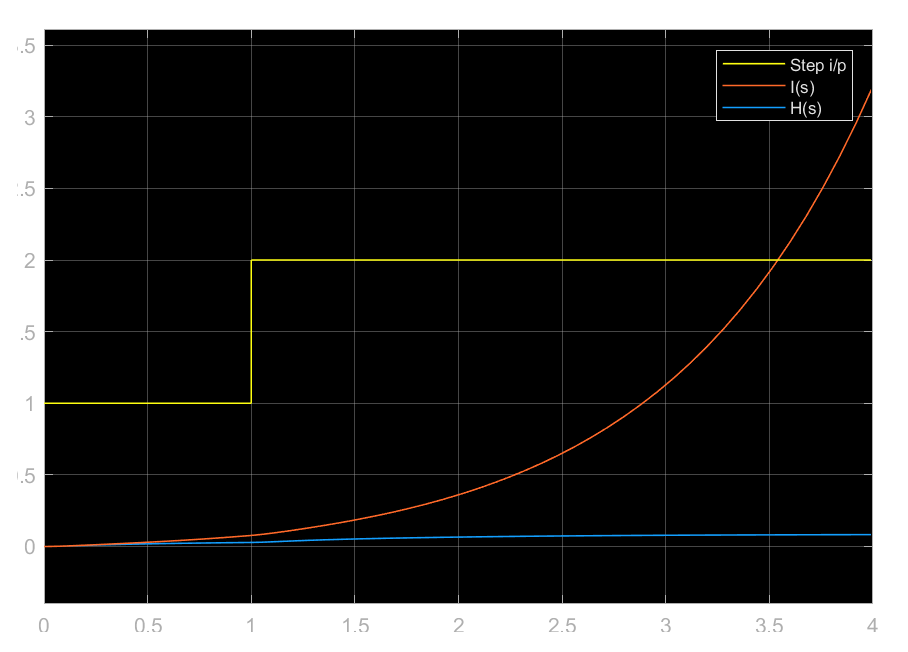
\includegraphics[width=\linewidth]{transfer_functions.eps}
    \caption{Modeling a simple input-output system, a stable step response and an unstable step response in voltage vs time in milliseconds.}
    \label{fig:transfer functions}
\end{figure}

\subsubsection{The roots and poles}

Given the transfer function 
\[
    H\brao*s = \frac{s^2 + 10s + 24}{s^4 + 26s^3 + 231s^2 + 766s + 560}\rlap,
\]
we find that the poles are in
\[
    \brac*{
        \begin{matrix}
            -10.0000 \\*
            -8.0000 \\*
            -7.0000 \\*
            -1.0000 \\*
        \end{matrix}
    }
\]
and the zeroes are in
\[
    \brac*{
        \begin{matrix}
            -6.0000 \\*
            -4.0000 \\*
        \end{matrix}
    }\rlap.
\]

Further, we modify this transfer function by negating the pole with the least magnitude ($-1.0000$) producing
\[
    I\brao*s = \frac{s^2 + 10 s + 24}{s^4 + 24 s^3 + 181 s^2 + 354 s - 560}\rlap.
\]

The result can be seen in Fig. \ref{fig:transfer functions}.

The step function jumps at $\SI1{\milli\second}$.
By $\SI3{\milli\second}$, $H\brao*s$ has settled at about $\SI1\volt$.
However, $I\brao{s}$ is at $\SI{1.129}\volt$ and goes beyond $\SI2\volt$ at time $\SI{3.543}{\milli\second}$.
It continues to grow exponentially.
This happens because $H\brao*s$ is a stable transfer function whereas $I\brao*s$ is unstable.

\section{Discussion}

This experiment was straightforward in its procedure.
We learned about how Matlab handles multiplication of polynomials,
and we also experienced a transfer function responding to a signal in a simulated system.

This experiment introduced the idea of stable and unstable transfer functions.
A stable transfer function can be used to attenuate a signal before it gets too far out of bounds.
However, an unstable function may not help with this.

Engineers may have more precise formulas to help choose the correct poles and zeros and properly design a transfer function.


\newpage
\appendix
\title{Appendix}\label{doc:apx}
\maketitle

\section{Part 1 -- Poles and zeroes, Matlab Live Script}

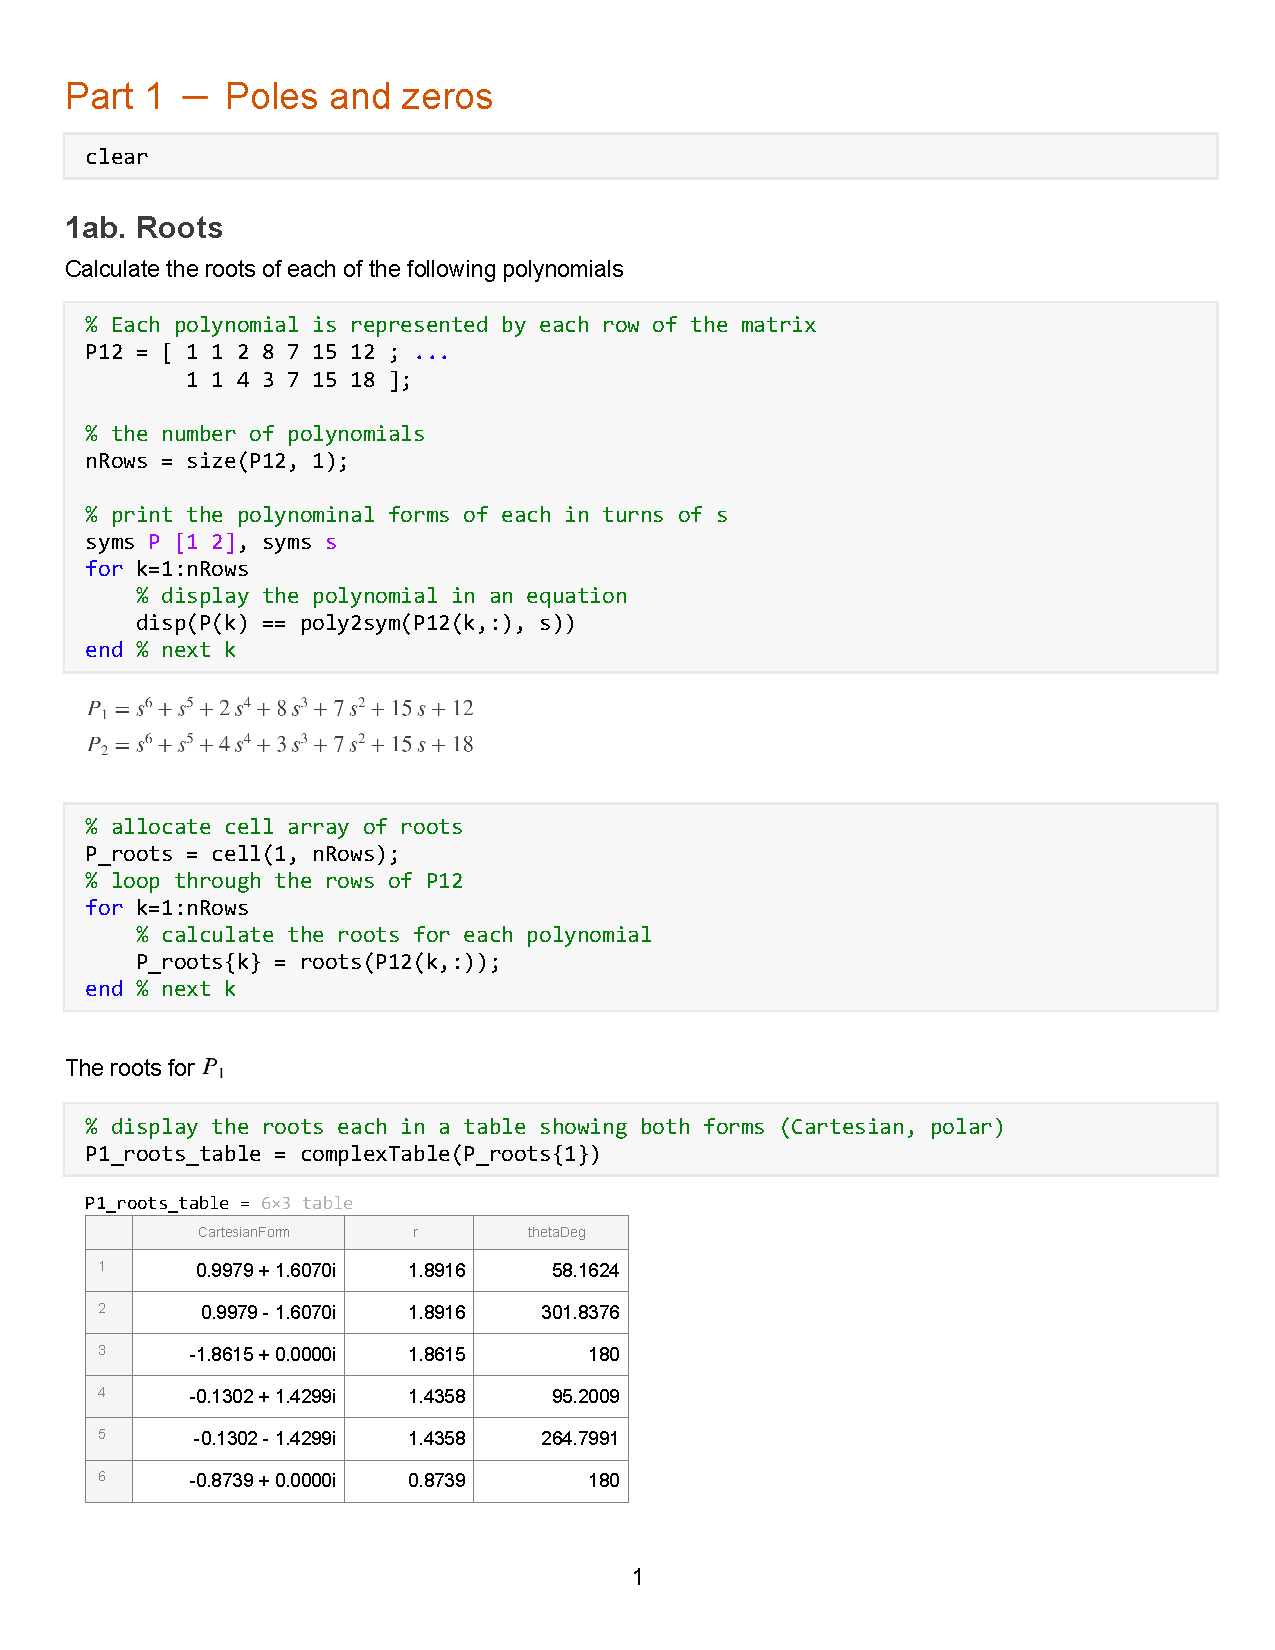
\includepdf[pages={-}]{part01_poles_zeros_mlx.pdf}

\section{Part 2 -- Laplace transforms, Matlab Live Script}

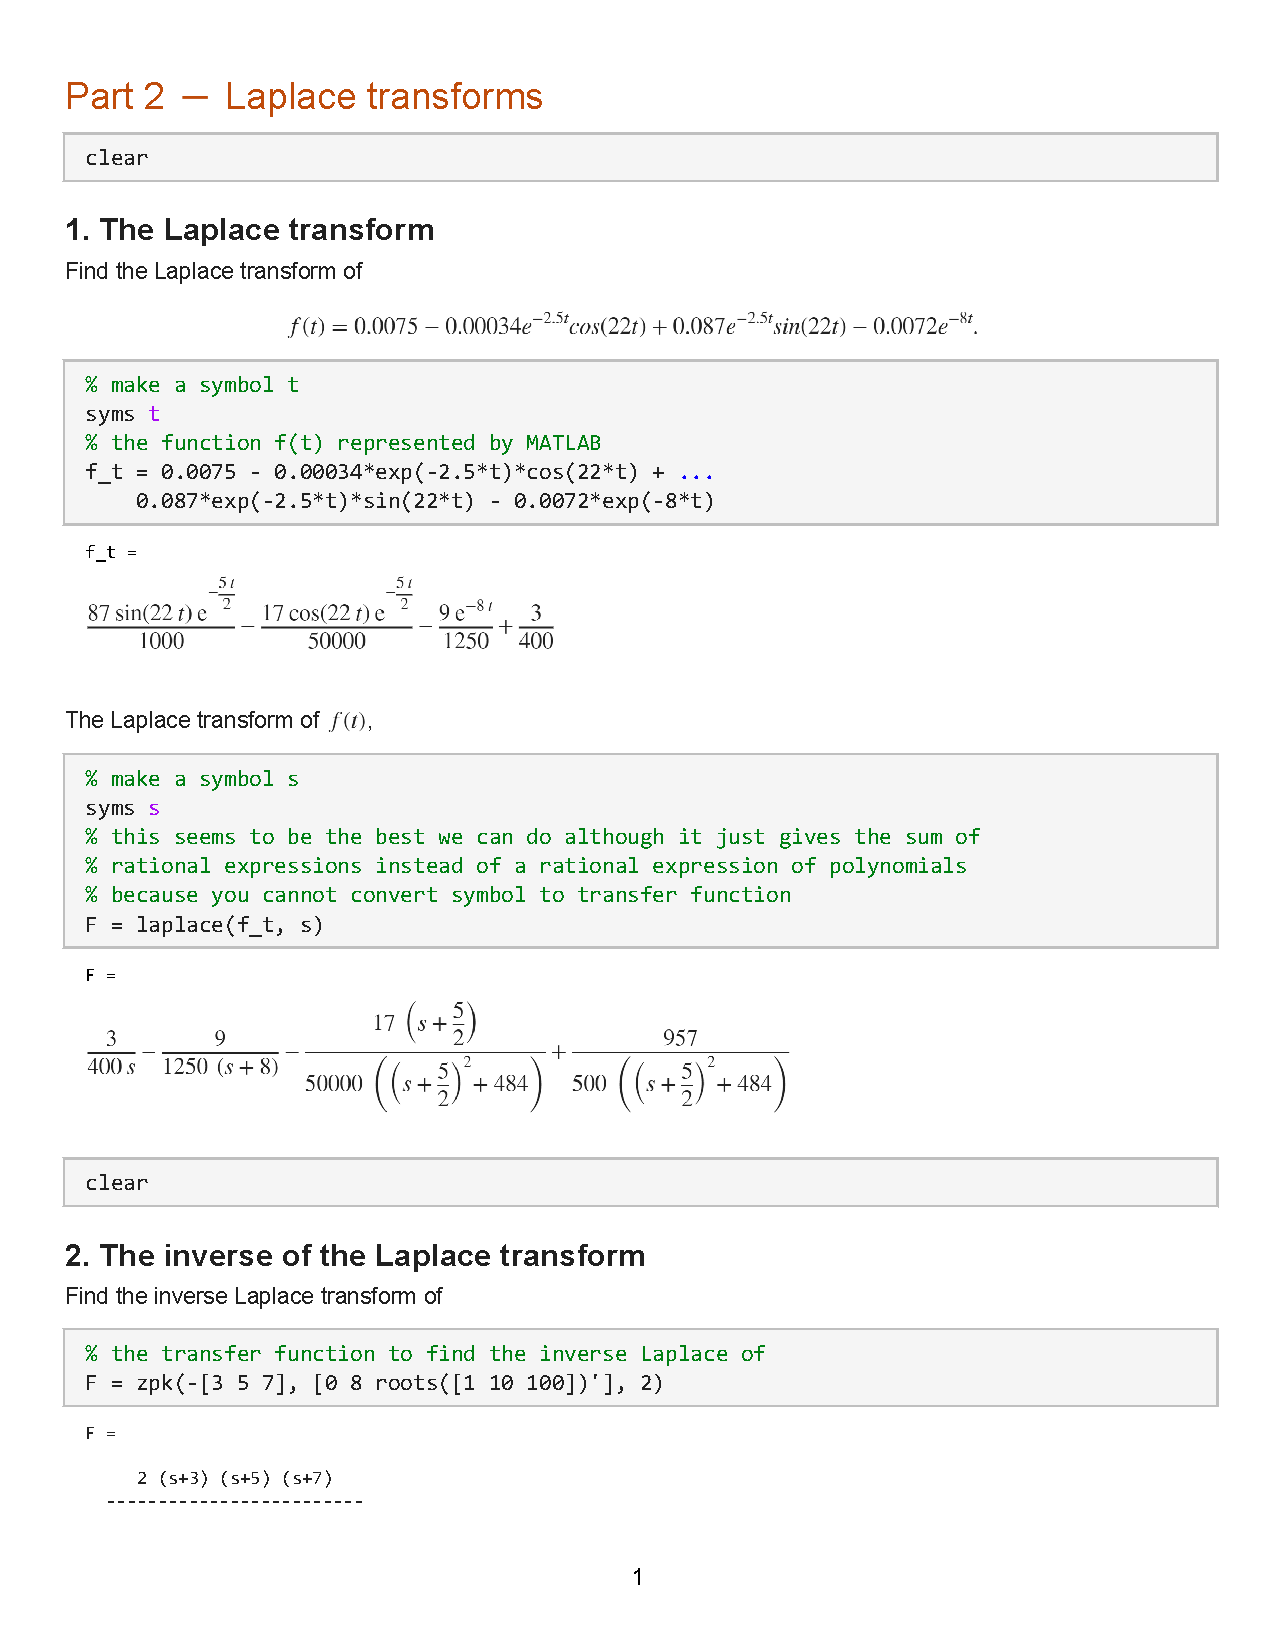
\includepdf[pages={-}]{part02_laplace_transforms_mlx.pdf}

\end{document}
